\documentclass{beamer}
\usetheme{metropolis}
\usepackage{graphicx}
\usepackage{amsmath}
\usepackage{makecell}
\usepackage{subfig}
\title{A History of Science in Latin America (INTD290): Unit 3.1}
\author{Jordan Hanson}
\institute{Whittier College Department of Physics and Astronomy}

\begin{document}
\maketitle

\section{Review}

\begin{frame}{Review}
\begin{enumerate}
\item \textbf{Unit 0} - \textit{Introduction}
\begin{itemize}
\item Introduction
\item Terminology - geographic, Catholic, Nahuatl, philosophical and scientific
\item What is Science
\end{itemize}
\item \textbf{Unit 1} - \textit{History of Science in Nueva Espa\~{n}a}
\begin{itemize}
\item Introduction - mining villages and HAWC
\item Timelines of mining guilds, founding of journals
\item Timelines of founding of colleges
\item Mexican discoveries in astronomy and solar physics
\end{itemize}
\item \textbf{Unit 2} - \textit{History of Science in Nueva Granada}
\begin{itemize}
\item Introduction - geocentrism versus heliocentrism
\item Scientific revolution and imporation to Columbia, Venezuela
\item Dominicans and Jesuits
\item Kepler's Laws
\item Pierre Auger Observatory and Cosmic Rays
\end{itemize}
\end{enumerate}
\end{frame}

\section{Summary}

\begin{frame}{Summary}
\begin{enumerate}
\item \textbf{Unit 3} - \textit{History of Science in R\'{i}o de La Plata and Exploration Literature}
\begin{itemize}
\item \alert{Three} groups of explorers explored R\'{i}o de La Plata and other sections of the colonies
\begin{itemize}
\item The Church
\item The Viceroyalty
\item The Crown or Home Country
\end{itemize}
\item General academic area of \textit{exploration literature}
\begin{itemize}
\item Writing in the face of the unknown
\item How to deal with latitude and longitude - \textit{Expedici\'{o}n Bot\'{a}nica, y La Condamine}
\item Expeditions to Latin America, and Antarctica\footnote{Return to Venus transit mission of Captain Cook, Tahiti, and Antarctica.}
\end{itemize}
\item The Atacama Large Millimeter/Sub-millimeter Array (ALMA)
\end{itemize}
\end{enumerate}
\end{frame}

\section{Exploration of R\'{i}o de La Plata}

\begin{frame}{Exploration of R\'{i}o de La Plata}
\begin{figure}
\centering
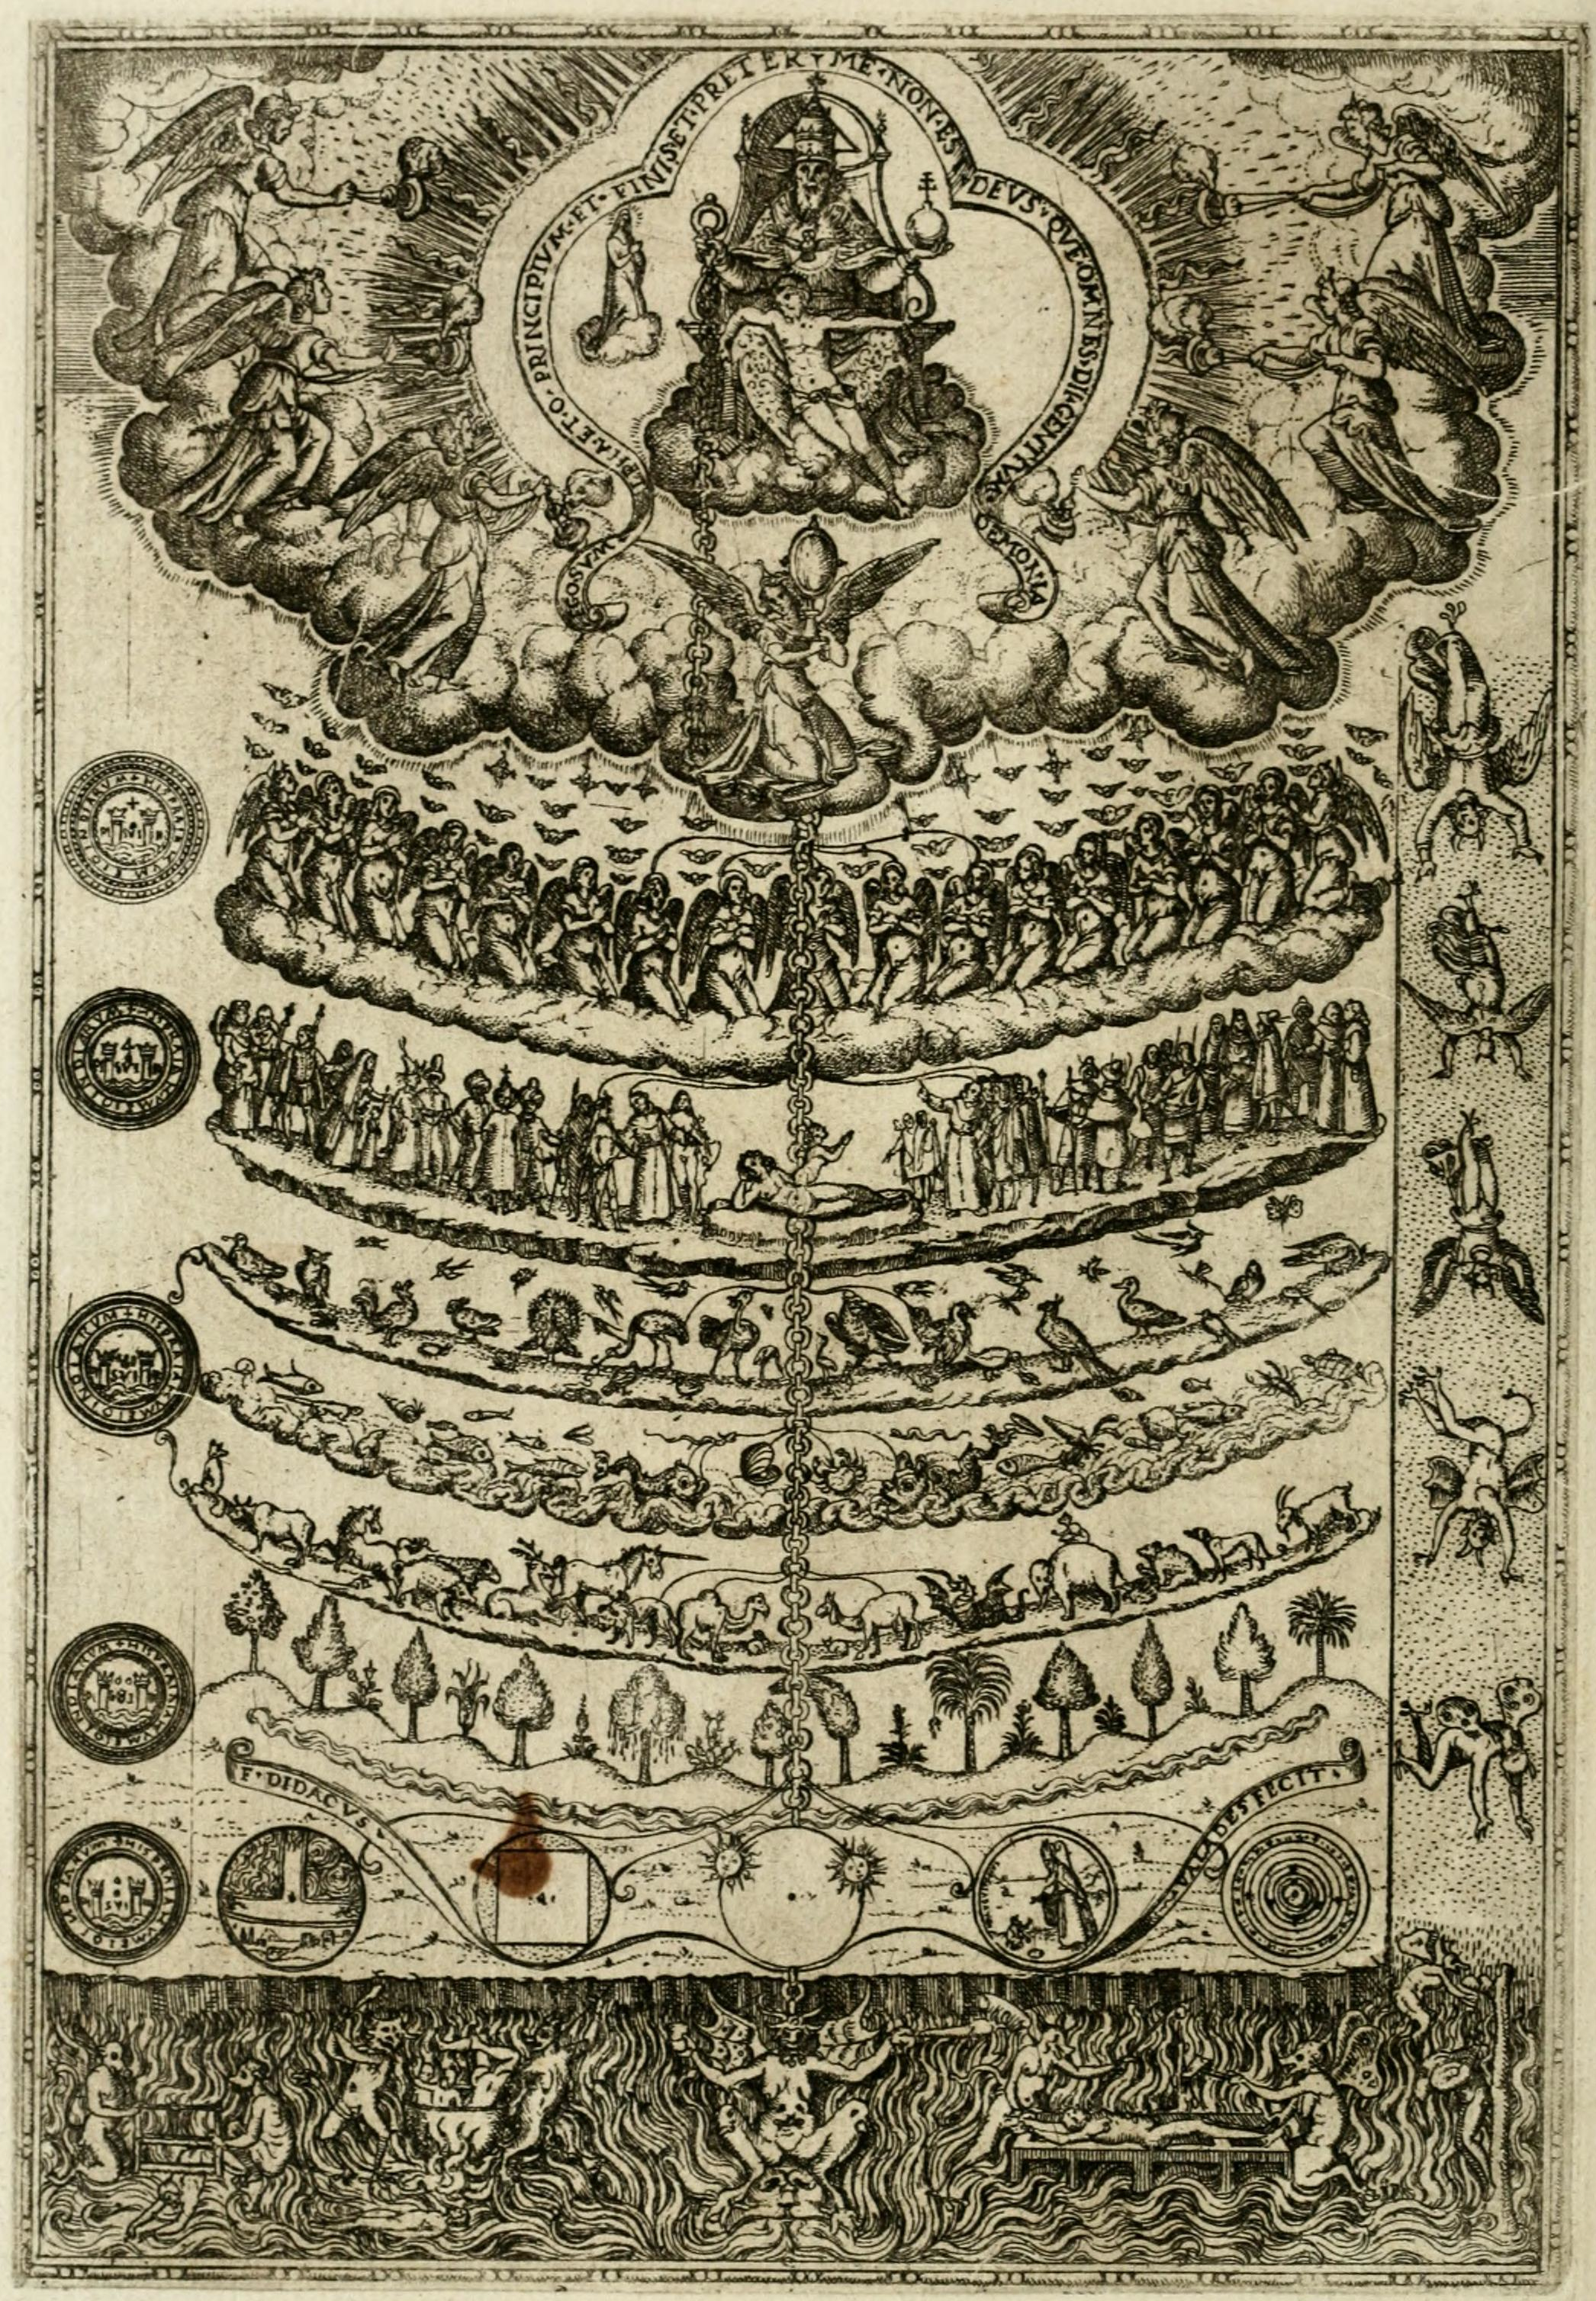
\includegraphics[width=4.5cm]{figures/chain.png}
\caption{The great chain of being.}
\end{figure}
\end{frame}

\begin{frame}{Exploration of R\'{i}o de La Plata}
\small
\begin{figure}
\centering
\includegraphics[width=9cm]{figures/lab.png}
\caption{The great chain of being - Jos\'{e} S\'{a}nchez Labrador.}
\end{figure}
\textit{Exploration of R\'{i}o de La Plata} for 30 years, Jesuit missionary
\begin{itemize}
\item Reopened communication between Potos\'{i} and Paraguay, alternative to route on Chaco river through Tucum\'{a}n. Re-connecting isolated mission in \textit{Chiquitos} via Paraguay river
\item Wrote \textit{Diario o relaci\'{o}n fragmentaria de los viajes desde la Reducci\'{o}n de Nuestra Se\~{n}ora de Bel\'{e}n hasta las misines de los Chiquitas, 1766-1767}
\end{itemize}
\end{frame}

\begin{frame}{Exploration of R\'{i}o de La Plata}
\small
\begin{figure}
\centering
\includegraphics[width=9cm]{figures/lab.png}
\caption{The great chain of being - Jos\'{e} S\'{a}nchez Labrador.}
\end{figure}
\textit{Exploration of R\'{i}o de La Plata} for 30 years, Jesuit missionary
\begin{itemize}
\item Mapped Paraguay river between 15 and 25 degrees South latitude
\item Completed \textit{Encyclopedia rioplatense} in Rome where he died
\begin{itemize}
\item \textit{Paraguay natural} - Natural history, botany (and \textit{ethnobotany}), zoological classification
\item \textit{Paraguay cultivado} - Agronomy
\item \textit{Paraguay cat\'{o}lico} - Human geography
\end{itemize}
\end{itemize}
\end{frame}

\begin{frame}{Exploration of R\'{i}o de La Plata}
\begin{figure}
\centering
\includegraphics[width=6cm]{figures/granChaco.jpg}
\includegraphics[width=4.5cm]{figures/rivers.png}
\caption{Rivers in South America.}
\end{figure}
\end{frame}

\section{Vectors and Distance}

\begin{frame}{Vectors and Distance}
Physics requires \alert{mathematical objects} to build equations that capture the behavior of nature.  Two examples of such objects are \alert{scalar} and \alert{vector} quantities.  Each type of object obeys similar but different rules.
\begin{enumerate}
\item Scalar quantities
\begin{itemize}
\item mass: $m_1+(m_2+m_3) = (m_1+m_2)+m_3$
\item speed: $v_1(v_2+v_3) = v_1v_2+v_1v_3$
\item charge: $q_1 \left(\frac{1}{q_1}\right) = 1$, $q_1(0) = 0$
\end{itemize}
\item Vector quantities
\begin{itemize}
\item velocity: $\vec{v}_1 + (\vec{v}_2+\vec{v}_3) = (\vec{v}_1 + \vec{v}_2)+\vec{v}_3$
\item tension: $\vec{t}_1 \cdot (\vec{t}_2 + \vec{t}_3) = \vec{t}_1 \cdot \vec{t}_2 + \vec{t}_1 \cdot \vec{t}_3$
\end{itemize}
\end{enumerate}
\textbf{Professor: show how to break into components, connection to trigonometry.}
\end{frame}

\begin{frame}{Vectors and Distance}
A vector may be expressed as \textit{a list of scalars}: $\vec{v} = (4,2)$ (a vector with two \textit{components}), $\vec{u} = (3,4,5)$ (three \textit{components}).  Now, we know how to add and subtract scalars.  How do we add and subtract vectors? \\
\vspace{0.5cm}
What is\\
$(1,3,8)+$\\ $(0,2,1)$? \\
Answer: $(1,5,9)$ \\
\vspace{0.5cm}
In other words, when adding vectors, we add them component by component. \textbf{Professor: work several examples.}
\end{frame}

\begin{frame}{Vectors and Distance}
How do we subtract vectors? In the same fashion:\\
\vspace{0.5cm}
What is\\
$(1,3,8)-$\\ $(0,2,1)$? \\
Answer: $(1,1,7)$ \\
\vspace{0.5cm}
In other words, when subtracting vectors, we subtract them component by component. \textbf{Professor: work several examples.}
\end{frame}

\begin{frame}{Vectors and Distance}
How do we multiply vectors? In the same fashion, \textit{for one kind of multiplication}:\\
\vspace{0.5cm}
What is\\
$(1,3,8)\cdot (0,2,1)$? \\
Answer: $1\cdot 0 + 3 \cdot 2 + 8 \cdot 1 = 14$ \\
\vspace{0.5cm}
\textit{This kind of multiplication is known as the dot-product}.  There is also the \textit{cross-product}, which we will save for later. \textbf{Professor: work several examples.}
\end{frame}

\begin{frame}{Vectors and Distance}
\small
The components of a vector may describe quantities in a \alert{coordinate system}, such as \textit{Cartesian coordinates} - after Ren\'e Descartes.  Vectors in the 3D Cartesian coordinate system (x,y,z) may be written in the following notation:
\\
\vspace{0.2cm}
$\boxed{\vec{v} = a\hat{i} + b\hat{j} + c\hat{k}}$
\\
\begin{itemize}
\item a: The amount in the +x-direction, $\hat{i}$: a vector of length 1, in the +x-direction
\item b: The amount in the +y-direction, $\hat{j}$: a vector of length 1, in the +y-direction
\item c: The amount in the +z-direction, $\hat{k}$: a vector of length 1, in the +z-direction
\end{itemize}
\end{frame}

\begin{frame}{Vectors and Distance}
\begin{figure}
\centering
\subfloat[\label{fig:twovectors_a}]{\includegraphics[width=0.45\textwidth,trim=1cm 1cm 1cm 1cm,clip=true]{figures/Vectors1.pdf}}
\subfloat[\label{fig:twovectors_b}]{\includegraphics[width=0.45\textwidth,trim=1cm 1cm 1cm 1cm,clip=true]{figures/Vectors2.pdf}}
\caption{\label{fig:twovectors} (a) Two vectors in a two-dimensional Cartesian coordinate system: $\vec{u} = 0.5\hat{i}+1.0\hat{j}$ and $\vec{v} = 2.0\hat{i}+1.0\hat{j}$.  (b) What is $\vec{u}+\vec{v}$?  Adding components: $\vec{u}+\vec{v} = 2.5\hat{i}+2.0\hat{j}$.}
\end{figure}
\end{frame}

\begin{frame}{Vectors and Distance}
\begin{figure}
\centering
\subfloat[\label{fig:twovectors_c}]{\includegraphics[width=0.45\textwidth,trim=1cm 1cm 1cm 1cm,clip=true]{figures/Vectors1.pdf}}
\subfloat[\label{fig:twovectors_d}]{\includegraphics[width=0.45\textwidth,trim=1cm 1cm 1cm 1cm,clip=true]{figures/Vectors3.pdf}}
\caption{\label{fig:twovectors2} (a) Two vectors in a two-dimensional Cartesian coordinate system: $\vec{u} = 0.5\hat{i}+1.0\hat{j}$ and $\vec{v} = 2.0\hat{i}+1.0\hat{j}$.  (b) What is $\vec{u}-\vec{v}$?  Subtracting components: $\vec{u}-\vec{v} = 1.5\hat{i}+0.0\hat{j}$.}
\end{figure}
\end{frame}

\begin{frame}{Vectors and Distance}
\begin{figure}
\centering
\subfloat[\label{fig:twovectors_e}]{\includegraphics[width=0.45\textwidth,trim=1cm 1cm 1cm 1cm,clip=true]{figures/Vectors1.pdf}}
\subfloat[\label{fig:twovectors_f}]{\includegraphics[width=0.45\textwidth,trim=1cm 1cm 1cm 1cm,clip=true]{figures/Vectors4.pdf}}
\caption{\label{fig:twovectors3} (a) Two vectors in a two-dimensional Cartesian coordinate system: $\vec{u} = 0.5\hat{i}+1.0\hat{j}$ and $\vec{v} = 2.0\hat{i}+1.0\hat{j}$.  (b) To compute $\vec{w}-\vec{v}$, arrange the vectors to get a sense of the result, $\vec{u}$.}
\end{figure}
\end{frame}

\begin{frame}{Vectors and Distance}
\small
\begin{minipage}[b]{0.45\linewidth}
$\vec{p} = 4\hat{i}+2\hat{j}$.  $\vec{q} = -4\hat{i}+2\hat{j}$.  \\
Compute $\vec{p} \cdot \vec{q}$.
\vspace{0.2cm}
\begin{itemize}
\item A: 12
\item B: -12
\item C: 4
\item D: 8
\end{itemize}
\end{minipage}
\hspace{0.5cm}
\begin{minipage}[b]{0.45\linewidth}
$\vec{p} = -1\hat{i}+6\hat{j}$.  $\vec{q} = 3\hat{i}+0.5\hat{j}$.  \\
Compute $\vec{p} \cdot \vec{q}$.
\vspace{0.2cm}
\begin{itemize}
\item A: -1
\item B: 1
\item C: 0
\item D: 3
\end{itemize}
\end{minipage}
\end{frame}

\begin{frame}{Vectors and Distance}
Why was the last answer zero?  Look at it graphically:
\begin{figure}
\centering
\includegraphics[width=0.5\textwidth,trim=1cm 1cm 1cm 1cm,clip=true]{figures/Vectors5.pdf}
\caption{\label{fig:twovectors4} Two vectors $\vec{p}$ and $\vec{q}$ are \textit{orthogonal} if $\vec{p} \cdot \vec{q} = 0$.}
\end{figure}
\end{frame}

\begin{frame}{Vectors and Distance}
What if the vectors are parallel? Look at it graphically:
\begin{figure}
\centering
\includegraphics[width=0.5\textwidth,trim=1cm 1cm 1cm 1cm,clip=true]{figures/Vectors6.pdf}
\caption{\label{fig:twovectors5} Two vectors $\vec{p}$ and $\vec{q}$ are \textit{parallel} if $\vec{p} \cdot \vec{q}$ is maximal.}
\end{figure}
\end{frame}

\begin{frame}{Vectors and Distance}
The \textit{length} or \textit{norm} of a vector $\vec{v} = a\hat{i}+b\hat{j}$ is $|\vec{v}| = \sqrt{a^2+b^2}$.\\
\begin{figure}
\centering
\includegraphics[width=0.5\textwidth,trim=1cm 1cm 1cm 1cm,clip=true]{figures/Vectors7.pdf}
\caption{\label{fig:twovectors6} Computing the norm of a vector $\vec{p}$.}
\end{figure}
\end{frame}

\begin{frame}{Vectors and Distance}
\small
\begin{minipage}[b]{0.45\linewidth}
An object moves at 2 m/s at $\theta = 60^{\circ}$ with respect to the x-axis.  What is the velocity of the object?
\vspace{0.2cm}
\begin{itemize}
\item A: $(1\hat{i}$ + $1\hat{j})$  m/s
\item B: $(\sqrt{3}\hat{i}$ + $1\hat{j})$  m/s
\item C: $(\sqrt{3}\hat{i}$ + $\sqrt{3}\hat{j})$  m/s
\item D: $(1\hat{i}$ + $\sqrt{3}\hat{j})$  m/s
\end{itemize}
\end{minipage}
\hspace{0.5cm}
\begin{minipage}[b]{0.45\linewidth}
What is the dot product of this velocity with another velocity: 5 m/s along the x-axis?
\vspace{0.7cm}
\begin{itemize}
\item A: 1 (m/s)$^2$
\item B: 5 (m/s)$^2$
\item C: 10 (m/s)$^2$
\item D: 5 (m/s)
\end{itemize}
\end{minipage}
\end{frame}

\begin{frame}{Vectors and Distance}
Is it possible to multiply vectors and scalars?  Of course: $a_1\vec{p} = a_1p_x\hat{i}+a_1p_y\hat{j}$.\\
\vspace{0.2cm}
Also, multiplication properties still hold.  For example: $(a_1+a_2)\vec{p} = a_1\vec{p}+a_2\vec{p}$. \\
\vspace{0.2cm}
\small
A spacecraft moves at 400 m/s, at an angle of 30 degrees with respect to the x-axis.  If it fires two thrusters that boost the x-component and y-component of the velocity by 25\% and 50\%, respectively, what is the final velocity?
\begin{itemize}
\item A: $(433\hat{i}+300\hat{j})$ m/s
\item B: $(300\hat{i}+433\hat{j})$ m/s
\item C: 400 m/s
\item D: $(400\hat{i}+433\hat{j})$ m/s
\end{itemize}
\end{frame}

\begin{frame}{Vectors and Distance}
We define the \textit{position} of an object as a vector locating it in a given coordinate system.  The scalar \textit{distance} is the norm of the position vector, that is, the distance to to the origin. \\
\vspace{0.5cm}
Now we can introduce the concept of \alert{dislacement}: a vector describing a movement of an object.
\end{frame}

\begin{frame}{Vectors and Distance}
\begin{figure}
\centering
\includegraphics[width=0.52\textwidth]{figures/Vectors4.pdf}
\caption{\label{fig:displacement} Suppose an object moves from position $\vec{v}$ to $\vec{w}$.  In this case, the \alert{displacement} is $\vec{u}$. \textbf{Thus, the final position is the initial position, plus the displacement.}}
\end{figure}
\end{frame}

\begin{frame}{Vectors and Distance}
It follows that the \textit{displacement} is zero if the initial and final positions are the same, but the \textit{distance travelled} is not.\\
\vspace{0.2cm}
\small
Suppose a jet fighter travelling at 800 km per hour banks such that it flies in a circle of radius 0.5 km.  How long does it take to complete the circle?  What is the distance traveled, and what is the displacement?
\begin{itemize}
\item A: $2\pi$ km, 28 seconds, $2\pi$ km
\item B: $\pi$ km, 14 seconds, $\pi$ km
\item C: $\pi$ km, 28 seconds, $\pi$ km
\item D: $\pi$ km, 14 seconds, $0$ km
\end{itemize}
\end{frame}

\section{Exploration Literature}

\section{Expedici\'{o}n Bot\'{a}nica, y La Condamine}

\section{Longitude and Latitude}

\end{document}